\documentclass[a4paper,12pt]{article}
\usepackage[utf8]{inputenc}
\usepackage[T2A]{fontenc}
\usepackage[russian]{babel}
\usepackage{geometry}
\usepackage{amsmath}
\usepackage{graphicx}
\usepackage{listings}
\usepackage{xcolor}
\usepackage[nottoc]{tocbibind}
\usepackage{hyperref}

% Настройки страницы
\geometry{left=3cm,right=1.5cm,top=2cm,bottom=2cm}

% Цвета для листингов
\definecolor{codegreen}{rgb}{0,0.6,0}
\definecolor{codegray}{rgb}{0.5,0.5,0.5}
\definecolor{codepurple}{rgb}{0.58,0,0.82}
\definecolor{backcolour}{rgb}{1.0,1.0,1.0}

\lstdefinestyle{mystyle}{
    backgroundcolor=\color{backcolour},
    commentstyle=\color{codegreen},
    keywordstyle=\color{blue},
    numberstyle=\tiny\color{codegray},
    stringstyle=\color{codepurple},
    basicstyle=\footnotesize,
    breakatwhitespace=false,
    breaklines=true,
    captionpos=b,
    keepspaces=true,
    numbers=left,
    numbersep=5pt,
    showspaces=false,
    showstringspaces=false,
    showtabs=false,
    tabsize=2
}

\lstset{style=mystyle}

% Центрирование текста
\newcommand{\centered}[1]{\begin{center}#1\end{center}}
\makeatletter
\renewenvironment{thebibliography}[1]
     {\section*{\refname} % Это создает заголовок — можно закомментировать
      \@mkboth{\MakeUppercase\refname}{\MakeUppercase\refname}
      \list{\@biblabel{\@arabic\c@enumiv}}%
           {\settowidth\labelwidth{\@biblabel{#1}}%
            \leftmargin\labelwidth
            \advance\leftmargin\labelsep
            \@openbib@code
            \usecounter{enumiv}%
            \let\p@enumiv\@empty
            \renewcommand\theenumiv{\@arabic\c@enumiv}%
            \setlength{\itemsep}{-0.5em}}
     \sloppy
     \clubpenalty4000
     \@clubpenalty \clubpenalty
     \widowpenalty4000%
     \sfcode`\.\@m}
     {\def\@noitemerr
       {\@latex@warning{Запись без \protect\bibitem}}
      \endlist}
\makeatother
\begin{document}



\thispagestyle{empty} % Убираем номер страницы на титульном листе

\centered{
{МИНИСТЕРСТВО НАУКИ И ВЫСШЕГО ОБРАЗОВАНИЯ \\
РОССИЙСКОЙ ФЕДЕРАЦИИ} \\[0cm]

Федеральное государственное бюджетное образовательное учреждение \\
высшего образования \\[0cm]

\textbf{АДЫГЕЙСКИЙ ГОСУДАРСТВЕННЫЙ УНИВЕРСИТЕТ} \\[0.3cm]

Инженерно-физический факультет \\
Кафедра автоматизированных систем обработки информации и управления
}

\vspace*{3cm}

\begin{center}
{Отчет по практике} \\[0.5cm]
\fontsize{20}{24}\selectfont{Программная реализация численного метода} \\[0cm]
\textit{Решение системы линейных алгебраических уравнений методом Гаусса-Жордана.}
\end{center}
\vspace*{0cm}

\begin{center}
1 курс, группа УТС1
\end{center}

\vspace*{1cm}

\begin{flushright}
\hspace*{2cm} % Отступ от правого края — регулируй по желанию
Выполнил: \\
\underline{\hspace{4cm}} \quad А.А. Сокур \\
\underline{«\hspace{0.8cm}»} \underline{\hspace{4cm}} 2025 г. \\
Руководитель: \\
\underline{\hspace{3.5cm}} \quad С.В. Теплоухов \\
\underline{«\hspace{0.8cm}»} \underline{\hspace{4cm}} 2025 г.
\end{flushright}

\vspace*{\fill}

\centered{
Майкоп, 2025 г.
}
\newpage


\section*{1. Введение}
\subsection*{1.1 Цель работы}
Цель работы — реализовать программу, решающую систему линейных алгебраических уравнений методом Гаусса–Жордана. Метод заключается в полном исключении неизвестных, приводя матрицу к единичному виду.

\section*{2 Ход работы}
\subsection*{2.1 Пример кода, решающего данную задачу}
\lstinputlisting{Spr1.cpp} % <-- сюда будет подключен ваш C++ файл

\subsection*{2.2 Формулы и описание метода}
Метод Гаусса–Жордана представляет собой модификацию классического метода Гаусса. Он заключается в том, чтобы привести расширенную матрицу к \textit{единичной форме}, после чего решение находится в последнем столбце.

Для каждого шага $ i $ выполняется следующее:
\begin{enumerate}
    \item Выбор ведущего элемента.
    \item Перестановка строк, если нужно.
    \item Нормализация строки по ведущему элементу.
    \item Обнуление всех других элементов в текущем столбце.
\end{enumerate}

\section*{3 Интерфейс программы}
 Реализация программы: решение системы линейных алгебраических уравнений методом Гаусса-Жордана.

\begin{figure}[h]
    \centering
    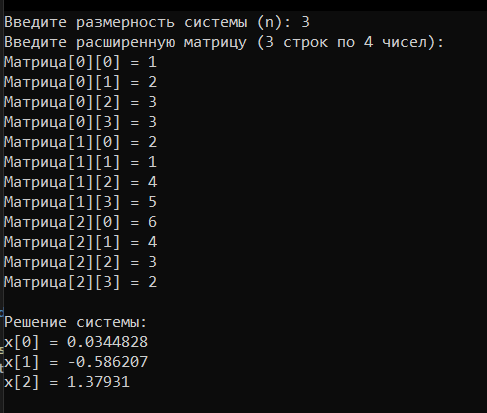
\includegraphics[width=0.7\linewidth]{sh1.png}
    \caption{Скриншот программы в консоли}
    \label{fig:sh1}
\end{figure}

На рисунке~\ref{fig:sh1} представлено окно командной строки с результатом выполнения программы.

\section*{Заключение}
В ходе выполнения лабораторной работы была реализована программа, решающая систему линейных алгебраических уравнений методом Гаусса–Жордана. Реализован контроль вводимых данных, а также оформлен отчёт.
\newpage
\addcontentsline{toc}{section}{Список литературы}

\begin{thebibliography}{8}
\bibitem{1} Бахвалов Н.С., Жидков Н.П., Кобельков Г.М. Численные методы. — Москва: Лаборатория Базовых Знаний, 2002 г.
\bibitem{2} Лафанов В.А. Программирование на языке C++. — Санкт-Петербург: Питер, 2018 г.
\end{thebibliography}

\end{document}